\section{Proposed Digitally Assisted Analog Front-End}
\label{sec:platform-design}

The proposed DA-AFE combines a conventional analog acquisition path with non-intrusive embedded digital assistance during foreground calibration. Unlike post-acquisition digital compensation, the embedded resources only establish the desired operating point of each analog stage; once calibration is completed they are disabled and acquisition proceeds entirely through the calibrated analog path.

The DA-AFE is implemented on a PSoC 5LP programmable mixed-signal platform. During foreground calibration, the embedded analog multiplexer, delta-sigma ADC, programmable digital filter, voltage DACs (VDACs), and embedded processor are non-intrusively repurposed as a mixed-signal feedback system that assists the analog circuitry while leaving the acquisition signal path unchanged. During normal operation, these resources resume their conventional acquisition functions.

The analog signal path, derived from the low-frequency geophone front end proposed by Ma \emph{et al.} \cite{Ma2023}, is shown in Fig.~\ref{fig:analog_path}. The conditioning chain consists of a programmable-gain instrumentation amplifier (PGA), a band-pass filter, an inverting summing stage, and a second-order low-pass filter. Four independently controlled VDACs shift the operating point of each stage during foreground calibration. Each reference node is decoupled by a 1~$\mu$F$\,\|\,$100~nF network that, together with the 16~k$\Omega$ internal output resistance of the VDAC, forms a single-pole low-pass filter at approximately 9~Hz, attenuating the 750~nV/$\sqrt{\mathrm{Hz}}$ VDAC noise density above that frequency \cite{InfineonPSoC}.

\begin{figure*}[!t]
	\centering
	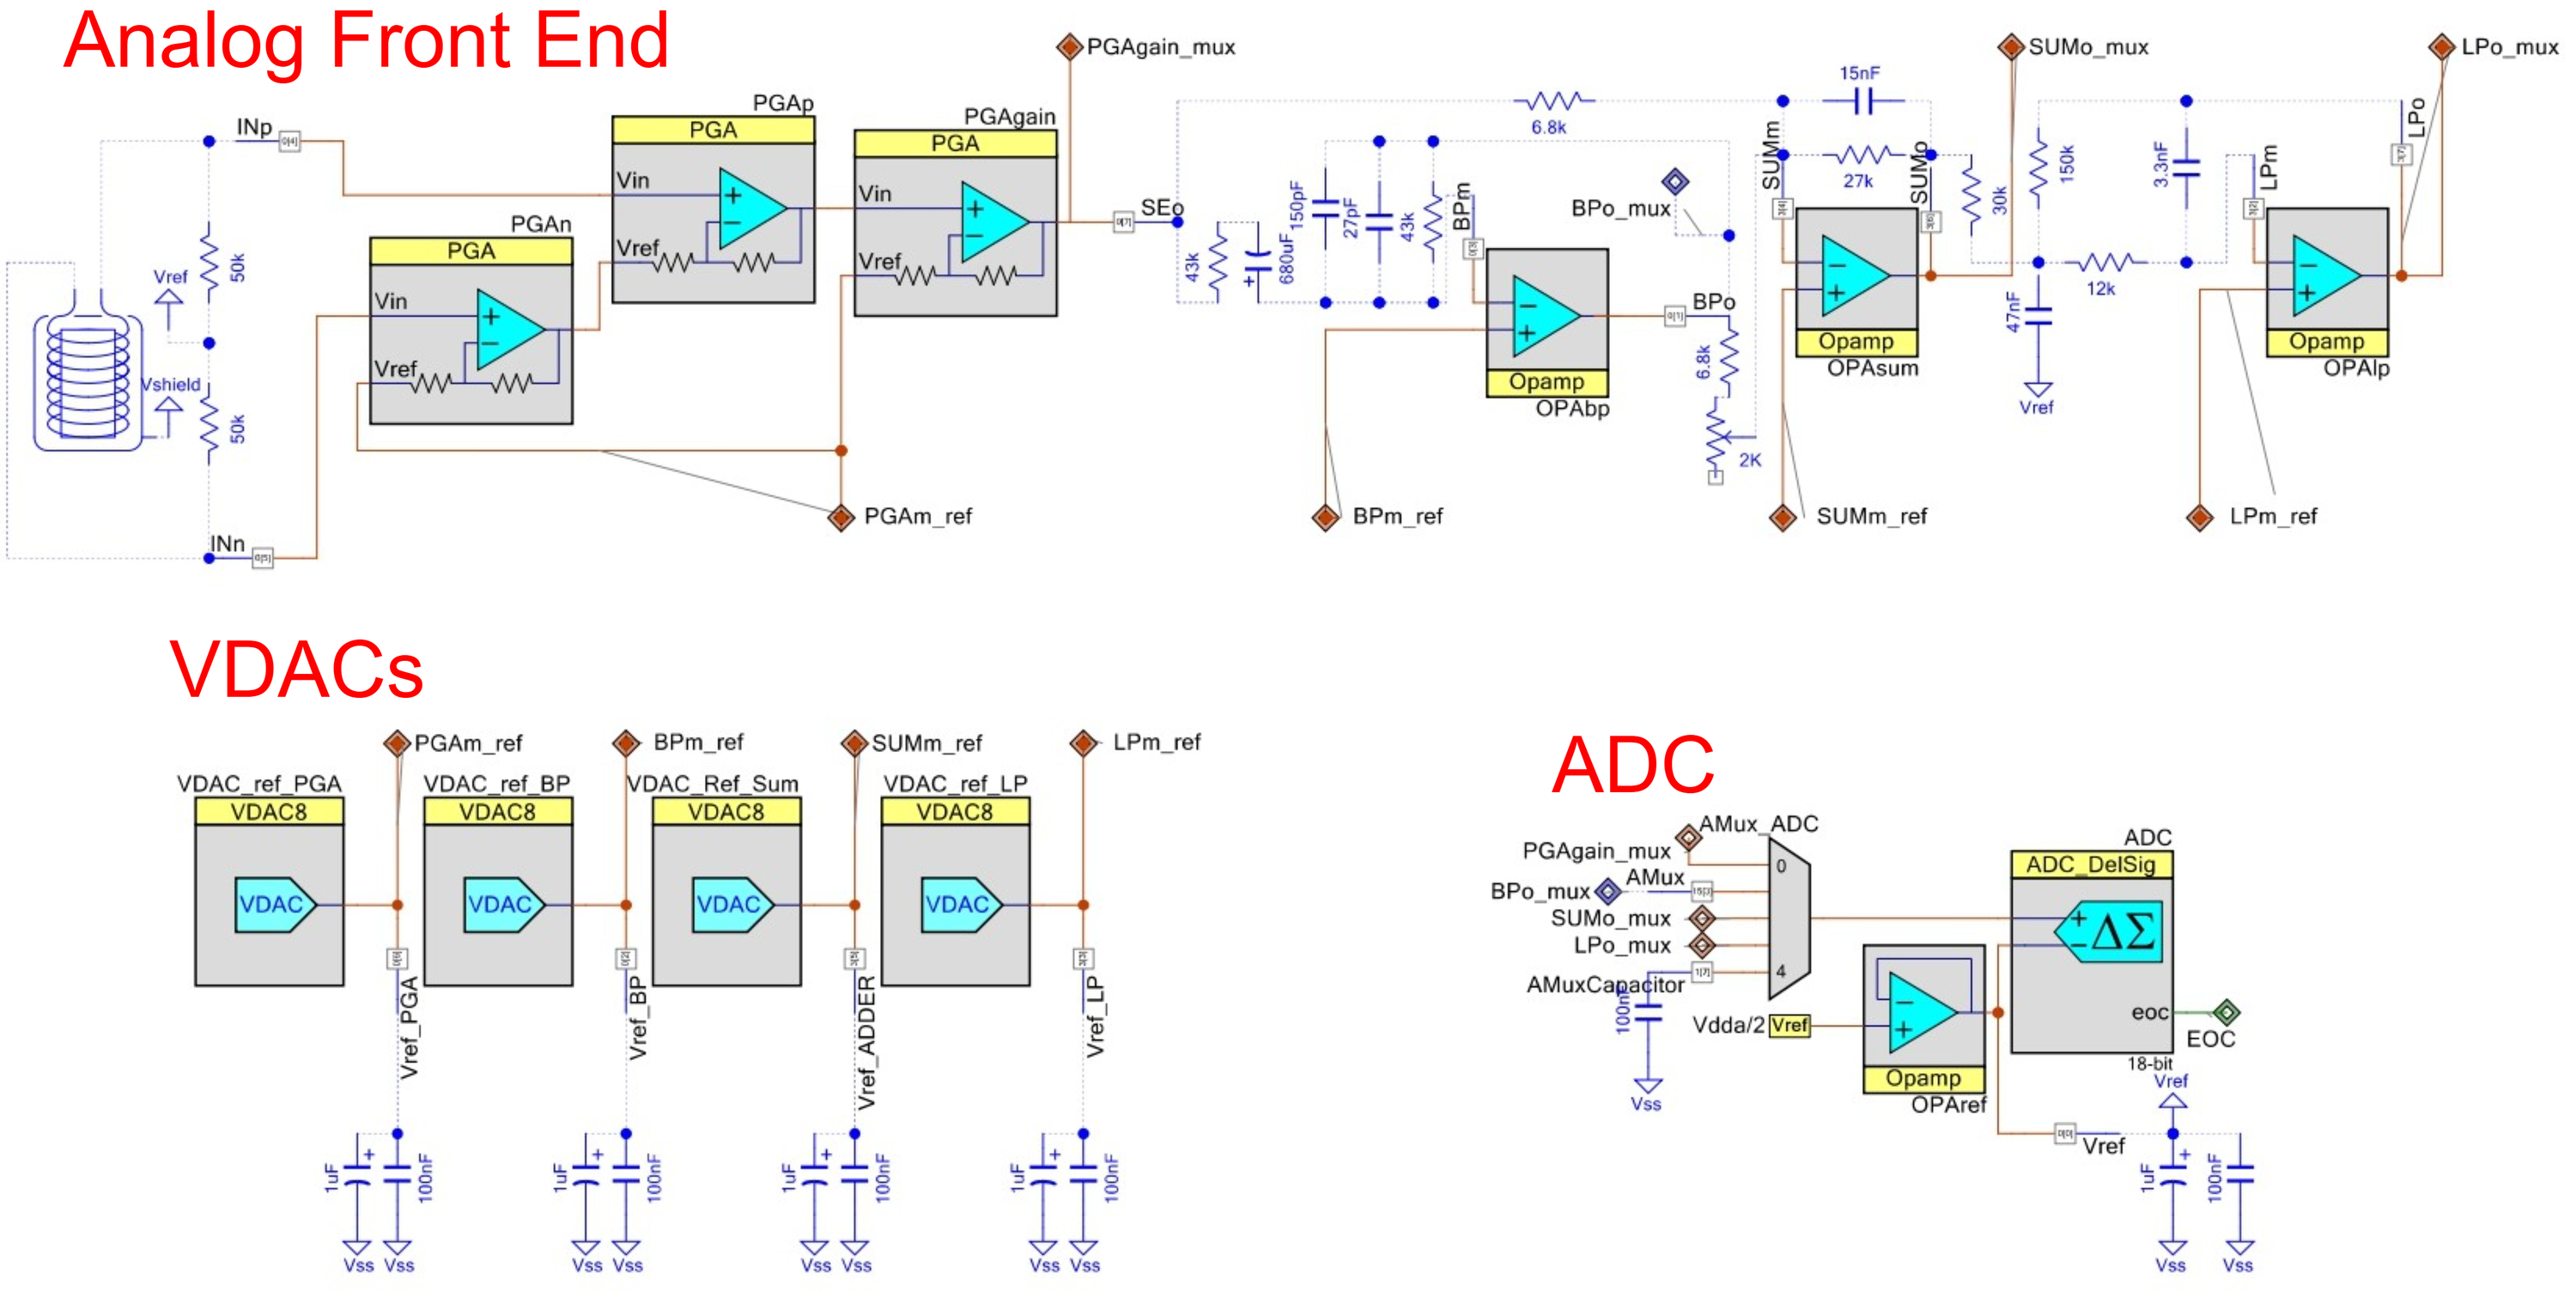
\includegraphics[width=1.00\textwidth]{imagenes/AnalogPathFinal_trim.png}
	\caption{Analog signal chain: four independent VDAC references trim the programmable-gain amplifier (PGA), band-pass filter (BP), summing stage (SUM), and low-pass filter (LP), with a shared ADC/multiplexer measurement path.}
	\label{fig:analog_path}
\end{figure*}

The embedded digital resources sequentially measure the output of each analog stage through the internal analog multiplexer and delta-sigma ADC. The filtered DC estimate determines the VDAC correction required to recenter each stage. Calibration proceeds from the PGA to the low-pass filter because each stage inherits the residual offset propagated from the preceding stages.

Assuming quasi-static offsets during calibration, negligible loading between stages, and linear superposition of DC contributions, the residual offset at the output of stage $i$ can be expressed as

\begin{equation}
 y_i^{\mathrm{DC}} =
 \sum_{j<i} A_{ij}y_j^{\mathrm{DC}}
 + b_i
 + K_i u_i,
 \label{eq:stage}
\end{equation}

where $A_{ij}$ represents the DC transfer gain from stage $j$ to stage $i$, $b_i$ denotes the intrinsic offset generated by stage $i$, and $K_i$ is the DC gain relating the injected VDAC voltage $u_i$ to the output of the corresponding stage.

This sequential operating principle is the key characteristic of the proposed DA-AFE: each stage is non-intrusively assisted until its operating point converges, after which the digital assistance is disabled and the analog front end operates as a conventional feed-forward signal chain throughout acquisition.
